% Section 11. Drafted from README.md ("Where the map stands"), REGIME-AUDIT.md and docs/COVERAGE.md.

\section{The regime map}\label{sec:map}

The results of \cref{sec:main,sec:crdt,sec:layer-a,sec:layer-c,sec:layer-b,sec:interfaces} are the
organizing core of a larger body of work: a map of the regimes of governed concurrent state. In every
regime it does not exclude by design, the map records a machine-checked exact condition, a proof that no efficient exact condition
exists unless $\mathrm{P} = \mathrm{NP}$, or an open problem listed in an audit. This section summarizes it (\cref{fig:atlas}, and by family in
\cref{app:map}); the regime-by-regime audit,
with the Coq theorem behind each entry, is part of the development.

\paragraph{Exact.} Single registries; causal and at-least-once delivery; CRDTs; stream processors;
acyclic federations of registries; a distributed propagation model, acyclic and on monotone cycles
with or without reset epochs; rootless propagation on every finite invertible network;
reconfiguration of a registry or a federation, at a barrier and live, under free, declared, causal
and at-least-once delivery; propagation over channels on acyclic networks, and with versioned merging
on every network in which each target has one source; and composition of blocks of any engines,
including cyclic monotone collapse.

\paragraph{Hard.} Consistency of a lossy network without a spanning root is NP-complete, by a
mechanized reduction from 3-SAT. Minimum coordination is characterized exactly and is NP-hard, from
Max-Cut on invertible networks and from 3-SAT on lossy ones.

\paragraph{Counting and gluing.} The first cohomology of the nerve is classified and counted over
$\mathbb{Z}/2$, and gluing local sections is exact on sub-federation covers; positive assembly of
local sections at the level of variables is narrowed but still open.

\paragraph{Open.} Seven convergence questions remain: rootless lossy networks, the distributed model
off its current hypotheses, rootless dynamics in which edges write values, existence of fixed points
in the resolver reading, distributed collapse of a cyclic block, reconfiguration with propagation in
flight, and versioned channels on networks with several sources or with cycles. Most concern cycles;
the audit states them as one question, what makes composition exact on cycles.

\paragraph{Excluded by design.} Least fixed points without the ascending chain condition, Byzantine
participants, nondeterministic repair, probabilistic schedules, infinite networks, and real-time
semantics.

\paragraph{Completeness of the map.} A coverage pass derived the space of regimes from the axes of the
model's premises and mapped every meaningful combination to the audit. The combinations no entry
covered became open problems or design exclusions; six of the seven open questions came from that
pass.

\begin{figure}[t]
\centering
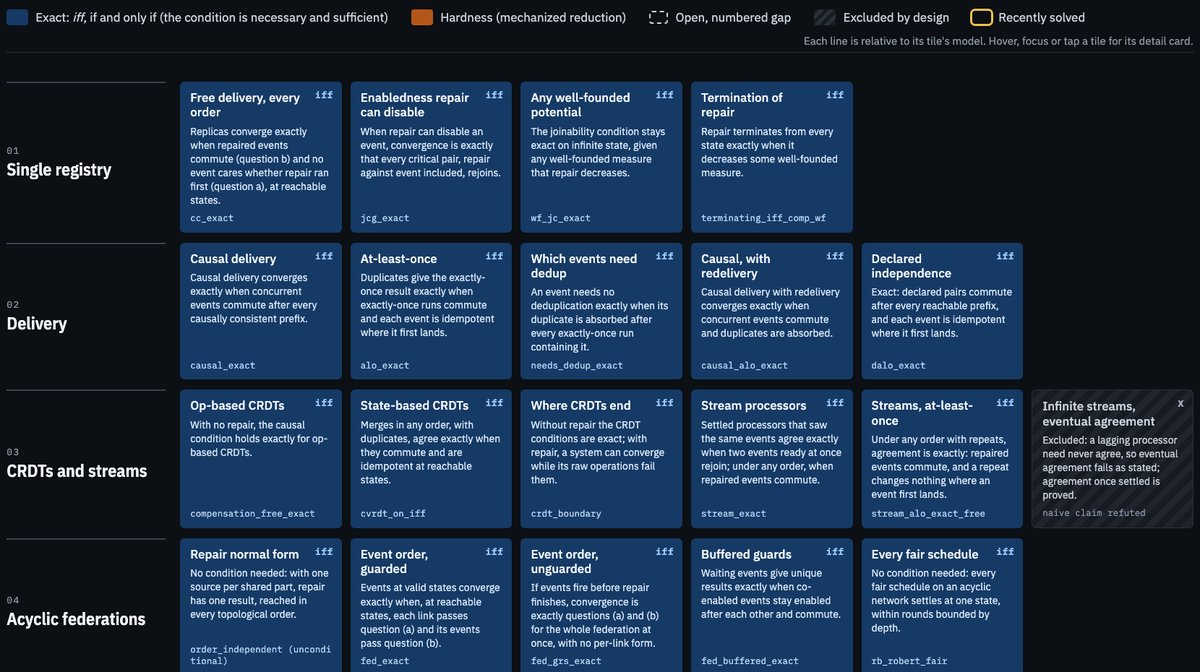
\includegraphics[width=\linewidth]{figures/atlas-preview.jpg}
\caption{Part of the Convergence Atlas: one tile per regime, grouped by family, each marked exact,
hard, open or excluded and linked to its theorem. The full atlas has 60 regimes in 11 families.}
\label{fig:atlas}
\end{figure}

\paragraph{Tiles and gaps.} The atlas has nine open tiles for the seven open convergence questions: one
question appears in two families, and one tile marks the open sheaf-assembly item above, which is not a
convergence question.

\paragraph{The evidence base.} The development's axiom-free gate checks 4{,}797 named results, every
one closed under the global context, with no axioms and no admitted proofs anywhere in the source, checked on three versions of Coq and Rocq on every change. The
counts are kept equal to the gate by a script that also checks every theorem name cited on the
atlas and the website against the source and the gate.
